\documentclass[11pt,a4paper]{article}
\usepackage[utf8]{inputenc}
\usepackage[english]{babel}
\usepackage{amsmath}
\usepackage{amsfonts}
\usepackage{amssymb}
\usepackage{graphicx}
\usepackage{listings}
\usepackage{xcolor}
\usepackage{booktabs}
\usepackage{tabularx}
\usepackage{array}
\usepackage{multirow}
\usepackage{tikz}
\usepackage{float}
\usepackage[margin=1in]{geometry}
\usepackage{hyperref}
\usetikzlibrary{shapes.geometric, arrows, positioning}

% Define colors for code listings
\definecolor{codegreen}{rgb}{0,0.6,0}
\definecolor{codegray}{rgb}{0.5,0.5,0.5}
\definecolor{codepurple}{rgb}{0.58,0,0.82}
\definecolor{backcolour}{rgb}{0.95,0.95,0.92}

% Code style for listings
\lstdefinestyle{code}{
    backgroundcolor=\color{backcolour},   
    commentstyle=\color{codegreen},
    keywordstyle=\color{magenta},
    numberstyle=\tiny\color{codegray},
    stringstyle=\color{codepurple},
    basicstyle=\ttfamily\footnotesize,
    breakatwhitespace=false,         
    breaklines=true,                 
    captionpos=b,                    
    keepspaces=true,                 
    numbers=left,                    
    numbersep=5pt,                  
    showspaces=false,                
    showstringspaces=false,
    showtabs=false,                  
    tabsize=2
}

\lstset{style=code}

\title{\textbf{MongoDB Schema Design for Northwind Database}\\
\large From E-Commerce Relational Model to Document-Oriented Architecture}

\author{Diogo Ribeiro\\
ESMAD - Instituto Politécnico do Porto\\
\texttt{dfr@esmad.ipp.pt}}

\date{\today}

\begin{document}

\maketitle

\begin{abstract}
This document presents a detailed analysis of transforming the Northwind Traders database from its traditional relational model to a MongoDB document-oriented schema. Northwind represents a classic e-commerce/trading company scenario with orders, products, customers, and suppliers. We explore three different schema design approaches, analyzing trade-offs between query performance, data consistency, and storage efficiency. The transformation demonstrates key NoSQL patterns including the Order-LineItems pattern, Product Catalog pattern, and Customer 360-view pattern, making it an ideal teaching example for NoSQL database courses.
\end{abstract}

\tableofcontents
\newpage

\section{Introduction}

The Northwind database has been a cornerstone of database education since its introduction by Microsoft. It models a food products trading company that manages orders between customers and suppliers across different categories of products. The database's moderate complexity (13 tables) and realistic business scenarios make it perfect for demonstrating MongoDB transformation patterns.

Unlike media rental systems (like Sakila) or music stores (like Chinook), Northwind represents core e-commerce patterns that are directly applicable to modern web applications. The challenge lies in optimizing for two competing access patterns: order processing (write-heavy) and business analytics (read-heavy).

\section{Original Relational Schema Analysis}

\subsection{Entity Overview}

The Northwind relational model consists of 13 interconnected tables:

\begin{table}[H]
\centering
\caption{Northwind Tables and Their Purpose}
\begin{tabularx}{\textwidth}{|l|X|r|l|}
\hline
\textbf{Table} & \textbf{Purpose} & \textbf{Row Count} & \textbf{Type} \\
\hline
Categories & Product classifications & 8 & Reference \\
Products & Product catalog & 77 & Core Entity \\
Suppliers & Product suppliers & 29 & Reference \\
Customers & Customer records & 91 & Core Entity \\
Employees & Staff members & 9 & Core Entity \\
Orders & Sales transactions & 830 & Transaction \\
Order\_Details & Line items in orders & 2,155 & Transaction \\
Shippers & Shipping companies & 3 & Reference \\
Territories & Sales territories & 53 & Reference \\
Region & Geographic regions & 4 & Reference \\
EmployeeTerritories & Employee assignments & 49 & Junction \\
CustomerDemographics & Customer categories & 0 & Reference \\
CustomerCustomerDemo & Customer categorization & 0 & Junction \\
\hline
\end{tabularx}
\end{table}

\subsection{Relationship Complexity}

The Northwind schema exhibits several relationship patterns:

\begin{itemize}
    \item \textbf{One-to-Many}: Customer $\rightarrow$ Orders, Order $\rightarrow$ OrderDetails
    \item \textbf{Many-to-One}: Product $\rightarrow$ Category, Product $\rightarrow$ Supplier
    \item \textbf{Many-to-Many}: Employee $\leftrightarrow$ Territory (via EmployeeTerritories)
    \item \textbf{Self-Referential}: Employee $\rightarrow$ Employee (ReportsTo hierarchy)
\end{itemize}

\section{MongoDB Schema Design Options}

\subsection{Design Approach 1: Order-Centric (Transaction-Focused)}

This approach optimizes for order processing and fulfillment workflows.

\begin{table}[H]
\centering
\caption{Order-Centric Schema Design}
\begin{tabularx}{\textwidth}{|l|X|X|}
\hline
\textbf{Collection} & \textbf{Embedded Data} & \textbf{References} \\
\hline
orders & order\_items[], customer snapshot, employee snapshot, shipper & None \\
products & category, supplier & None \\
customers & full address, contact info & None \\
employees & territories[], manager reference & manager\_id \\
\hline
\end{tabularx}
\end{table}

\subsection{Design Approach 2: Customer-Centric (360-View)}

This approach optimizes for customer service and relationship management.

\begin{table}[H]
\centering
\caption{Customer-Centric Schema Design}
\begin{tabularx}{\textwidth}{|l|X|X|}
\hline
\textbf{Collection} & \textbf{Embedded Data} & \textbf{References} \\
\hline
customers & recent\_orders[], lifetime\_stats & None \\
orders & order\_items[], shipping\_address & customer\_id, employee\_id \\
products & category, supplier, inventory\_stats & None \\
employees & territories[], reports\_to chain & None \\
\hline
\end{tabularx}
\end{table}

\subsection{Design Approach 3: Balanced Hybrid (Recommended)}

This approach balances operational and analytical needs.

\begin{table}[H]
\centering
\caption{Balanced Hybrid Schema Design}
\begin{tabularx}{\textwidth}{|l|X|X|}
\hline
\textbf{Collection} & \textbf{Embedded Data} & \textbf{References} \\
\hline
products & category, supplier & None \\
customers & address, demographics, order\_summary & None \\
orders & order\_items[], customer\_snapshot, totals & customer\_id, employee\_id \\
employees & territories[], full manager chain & None \\
\hline
\end{tabularx}
\end{table}

\section{Detailed Schema Implementation}

\subsection{Products Collection}

The products collection serves as the master catalog with embedded supplier and category information.

\begin{lstlisting}[caption={Products Collection Document Structure}]
{
  _id: ObjectId("..."),
  product_id: 1,
  product_name: "Chai",
  unit: "10 boxes x 20 bags",
  unit_price: 18.00,
  units_in_stock: 39,
  units_on_order: 0,
  reorder_level: 10,
  discontinued: false,
  
  // Embedded category (1:1 relationship)
  category: {
    category_id: 1,
    category_name: "Beverages",
    description: "Soft drinks, coffees, teas, beers, and ales"
  },
  
  // Embedded supplier (1:1 relationship)
  supplier: {
    supplier_id: 1,
    company_name: "Exotic Liquids",
    contact_name: "Charlotte Cooper",
    contact_title: "Purchasing Manager",
    address: {
      street: "49 Gilbert St.",
      city: "London",
      region: null,
      postal_code: "EC1 4SD",
      country: "UK"
    },
    phone: "(171) 555-2222"
  },
  
  // Computed fields for analytics
  analytics: {
    total_orders: 156,
    total_quantity_sold: 1874,
    total_revenue: 33732.00,
    avg_order_quantity: 12,
    last_ordered: ISODate("2024-01-15T00:00:00Z")
  }
}
\end{lstlisting}

\textbf{Design Justification:}
\begin{itemize}
    \item \textbf{Embedded Category}: Products never change categories, always displayed together
    \item \textbf{Embedded Supplier}: One primary supplier per product, frequently accessed
    \item \textbf{Analytics Fields}: Pre-computed for dashboard queries
    \item \textbf{Document Size}: Average 1-2KB, well within limits
\end{itemize}

\subsection{Customers Collection}

The customers collection provides a complete customer profile with order statistics.

\begin{lstlisting}[caption={Customers Collection Document Structure}]
{
  _id: ObjectId("..."),
  customer_id: "ALFKI",
  company_name: "Alfreds Futterkiste",
  contact_name: "Maria Anders",
  contact_title: "Sales Representative",
  
  // Embedded address (always needed together)
  address: {
    street: "Obere Str. 57",
    city: "Berlin",
    region: null,
    postal_code: "12209",
    country: "Germany",
    location: {
      type: "Point",
      coordinates: [13.32, 52.52] // [longitude, latitude]
    }
  },
  
  phone: "030-0074321",
  fax: "030-0076545",
  
  // Customer insights (computed periodically)
  insights: {
    customer_since: ISODate("1997-08-25T00:00:00Z"),
    total_orders: 6,
    total_spent: 4596.20,
    average_order_value: 766.03,
    last_order_date: ISODate("1998-04-09T00:00:00Z"),
    preferred_categories: ["Dairy Products", "Beverages"],
    lifetime_value_segment: "Gold",
    credit_limit: 5000.00,
    payment_terms: "Net 30"
  },
  
  // Recent activity (bounded array)
  recent_orders: [
    {
      order_id: 10835,
      order_date: ISODate("1998-01-15T00:00:00Z"),
      total: 845.80,
      status: "Delivered"
    }
    // ... last 5 orders only
  ],
  
  // Demographics (if applicable)
  demographics: {
    industry: "Food Service",
    company_size: "Small",
    annual_revenue: "1M-5M"
  }
}
\end{lstlisting}

\textbf{Design Justification:}
\begin{itemize}
    \item \textbf{Embedded Address}: Including GeoJSON for location-based queries
    \item \textbf{Customer Insights}: Pre-aggregated metrics for customer service
    \item \textbf{Recent Orders}: Bounded to last 5 for quick reference
    \item \textbf{Demographics}: Optional fields for B2B customers
\end{itemize}

\subsection{Orders Collection}

The orders collection captures complete transaction details with embedded line items.

\begin{lstlisting}[caption={Orders Collection Document Structure}]
{
  _id: ObjectId("..."),
  order_id: 10248,
  order_date: ISODate("1996-07-04T00:00:00Z"),
  required_date: ISODate("1996-08-01T00:00:00Z"),
  shipped_date: ISODate("1996-07-16T00:00:00Z"),
  
  // Customer snapshot at time of order
  customer: {
    customer_id: "VINET",
    company_name: "Vins et alcools Chevalier",
    contact_name: "Paul Henriot"
  },
  
  // Employee snapshot
  employee: {
    employee_id: 5,
    first_name: "Steven",
    last_name: "Buchanan",
    title: "Sales Manager"
  },
  
  // Embedded line items (the key pattern)
  order_items: [
    {
      line_number: 1,
      product: {
        product_id: 11,
        product_name: "Queso Cabrales",
        category_name: "Dairy Products"
      },
      unit_price: 14.00,
      quantity: 12,
      discount: 0.0,
      line_total: 168.00
    },
    {
      line_number: 2,
      product: {
        product_id: 42,
        product_name: "Singaporean Hokkien Fried Mee",
        category_name: "Grains/Cereals"
      },
      unit_price: 9.80,
      quantity: 10,
      discount: 0.0,
      line_total: 98.00
    }
  ],
  
  // Shipping information
  shipping: {
    ship_name: "Vins et alcools Chevalier",
    ship_address: {
      street: "59 rue de l'Abbaye",
      city: "Reims",
      region: null,
      postal_code: "51100",
      country: "France"
    },
    shipper: {
      shipper_id: 3,
      company_name: "Federal Shipping",
      phone: "(503) 555-9931"
    },
    freight: 32.38
  },
  
  // Order totals (pre-calculated)
  totals: {
    subtotal: 266.00,
    freight: 32.38,
    discount_amount: 0.00,
    total: 298.38,
    item_count: 2,
    total_quantity: 22
  },
  
  // Status tracking
  status: {
    current: "Delivered",
    payment_status: "Paid",
    fulfillment_status: "Complete",
    history: [
      {
        status: "Placed",
        timestamp: ISODate("1996-07-04T00:00:00Z"),
        notes: "Order received"
      },
      {
        status: "Shipped",
        timestamp: ISODate("1996-07-16T00:00:00Z"),
        notes: "Shipped via Federal Shipping"
      },
      {
        status: "Delivered",
        timestamp: ISODate("1996-07-18T00:00:00Z"),
        notes: "Delivered to customer"
      }
    ]
  }
}
\end{lstlisting}

\textbf{Design Justification:}
\begin{itemize}
    \item \textbf{Embedded Line Items}: Core to order, always accessed together
    \item \textbf{Customer/Employee Snapshots}: Historical accuracy, avoid joins
    \item \textbf{Pre-calculated Totals}: Faster reporting and analytics
    \item \textbf{Status History}: Audit trail and workflow tracking
\end{itemize}

\subsection{Employees Collection}

The employees collection handles organizational hierarchy and territory assignments.

\begin{lstlisting}[caption={Employees Collection Document Structure}]
{
  _id: ObjectId("..."),
  employee_id: 5,
  first_name: "Steven",
  last_name: "Buchanan",
  title: "Sales Manager",
  title_of_courtesy: "Mr.",
  birth_date: ISODate("1955-03-04T00:00:00Z"),
  hire_date: ISODate("1993-10-17T00:00:00Z"),
  
  // Contact information
  contact: {
    address: {
      street: "14 Garrett Hill",
      city: "London",
      region: null,
      postal_code: "SW1 8JR",
      country: "UK"
    },
    home_phone: "(71) 555-4848",
    extension: "3453"
  },
  
  // Organizational hierarchy
  organization: {
    reports_to: 2,
    manager: {
      employee_id: 2,
      name: "Andrew Fuller",
      title: "Vice President, Sales"
    },
    // Full chain for org chart queries
    management_chain: [
      {
        employee_id: 2,
        name: "Andrew Fuller",
        title: "Vice President, Sales"
      }
    ],
    direct_reports: [
      {
        employee_id: 6,
        name: "Michael Suyama",
        title: "Sales Representative"
      },
      {
        employee_id: 7,
        name: "Robert King",
        title: "Sales Representative"
      }
    ]
  },
  
  // Embedded territories
  territories: [
    {
      territory_id: "02116",
      territory_description: "Boston",
      region: "Eastern"
    },
    {
      territory_id: "02139",
      territory_description: "Cambridge",
      region: "Eastern"
    }
  ],
  
  // Performance metrics
  performance: {
    total_sales: 134507.00,
    total_orders: 123,
    average_order_value: 1093.54,
    current_month_sales: 12450.00,
    current_year_sales: 98234.00,
    customer_satisfaction: 4.8
  },
  
  // Additional information
  notes: "Steven Buchanan graduated from St. Andrews University...",
  photo_path: "/employees/photos/buchanan.jpg"
}
\end{lstlisting}

\textbf{Design Justification:}
\begin{itemize}
    \item \textbf{Management Chain}: Pre-computed for organizational queries
    \item \textbf{Direct Reports}: Bounded list for team management
    \item \textbf{Embedded Territories}: Small, stable set per employee
    \item \textbf{Performance Metrics}: Real-time KPIs for dashboards
\end{itemize}

\section{Query Pattern Analysis}

\subsection{Common Query Patterns and Their Implementation}

\begin{table}[H]
\centering
\caption{Query Pattern Performance Comparison}
\begin{tabularx}{\textwidth}{|X|c|c|c|}
\hline
\textbf{Query Pattern} & \textbf{Frequency} & \textbf{Joins Required} & \textbf{Performance} \\
\hline
Find products by category & Very High & 0 & Excellent \\
Get order with all details & Very High & 0 & Excellent \\
Customer order history & High & 1 (\$lookup) & Good \\
Product sales analytics & Medium & 1 (aggregation) & Good \\
Employee sales performance & Medium & 1 (aggregation) & Good \\
Inventory reorder report & Low & 0 & Excellent \\
Territory sales analysis & Low & 2 (aggregation) & Fair \\
\hline
\end{tabularx}
\end{table}

\subsection{Optimized Query Examples}

\begin{lstlisting}[caption={Common MongoDB Queries for Northwind}]
// 1. Find all beverages under $20
db.products.find({
  "category.category_name": "Beverages",
  "unit_price": { $lt: 20 }
})

// 2. Get complete order details (no join needed!)
db.orders.findOne({ order_id: 10248 })

// 3. Customer lifetime value
db.customers.findOne(
  { customer_id: "ALFKI" },
  { "insights.lifetime_value_segment": 1, 
    "insights.total_spent": 1 }
)

// 4. Products needing reorder
db.products.find({
  $expr: { 
    $lte: ["$units_in_stock", "$reorder_level"] 
  }
})

// 5. Monthly sales by employee
db.orders.aggregate([
  {
    $match: {
      order_date: {
        $gte: ISODate("1997-01-01"),
        $lt: ISODate("1997-02-01")
      }
    }
  },
  {
    $group: {
      _id: "$employee.employee_id",
      employee_name: { 
        $first: { 
          $concat: ["$employee.first_name", " ", 
                    "$employee.last_name"] 
        }
      },
      total_sales: { $sum: "$totals.total" },
      order_count: { $sum: 1 }
    }
  },
  { $sort: { total_sales: -1 } }
])

// 6. Top selling products
db.orders.aggregate([
  { $unwind: "$order_items" },
  {
    $group: {
      _id: "$order_items.product.product_id",
      product_name: { 
        $first: "$order_items.product.product_name" 
      },
      total_quantity: { 
        $sum: "$order_items.quantity" 
      },
      total_revenue: { 
        $sum: "$order_items.line_total" 
      }
    }
  },
  { $sort: { total_revenue: -1 } },
  { $limit: 10 }
])
\end{lstlisting}

\section{Trade-off Analysis}

\subsection{Storage Efficiency Analysis}

\begin{table}[H]
\centering
\caption{Storage Comparison Across Design Approaches}
\begin{tabularx}{\textwidth}{|l|X|X|X|}
\hline
\textbf{Metric} & \textbf{Normalized} & \textbf{Our Design} & \textbf{Fully Denormalized} \\
\hline
Collection Count & 13 & 4 & 1 \\
Document Count & $\sim$3,300 & $\sim$1,007 & $\sim$830 \\
Avg Document Size & 200B & 2KB & 15KB \\
Total Storage & $\sim$1MB & $\sim$3MB & $\sim$12MB \\
Data Duplication & None & Minimal & Significant \\
Index Count & 20+ & 12 & 5 \\
\hline
\end{tabularx}
\end{table}

\subsection{Update Complexity Matrix}

\begin{table}[H]
\centering
\caption{Update Operations Complexity}
\begin{tabularx}{\textwidth}{|X|c|c|c|}
\hline
\textbf{Update Scenario} & \textbf{Normalized} & \textbf{Our Design} & \textbf{Denormalized} \\
\hline
Change product price & 1 update & 1 update & Many updates \\
Update customer address & 1 update & 1 update & Many updates \\
Add order & 2+ inserts & 1 insert & 1 insert \\
Cancel order line item & 1 delete & 1 pull operation & 1 pull operation \\
Change category name & 1 update & Many updates & Many updates \\
Update employee territory & 1 update & 1 update & 1 update \\
\hline
\end{tabularx}
\end{table}

\subsection{Performance Characteristics}

\begin{table}[H]
\centering
\caption{Performance Metrics by Operation Type}
\begin{tabularx}{\textwidth}{|l|X|X|X|}
\hline
\textbf{Operation} & \textbf{Response Time} & \textbf{Complexity} & \textbf{Scalability} \\
\hline
Single order retrieval & $<$1ms & O(1) & Excellent \\
Product catalog search & $<$5ms & O(log n) & Excellent \\
Customer 360 view & $<$2ms & O(1) & Excellent \\
Order placement & $<$10ms & O(1) & Good \\
Sales analytics & $<$100ms & O(n) & Fair \\
Inventory update & $<$5ms & O(1) & Excellent \\
\hline
\end{tabularx}
\end{table}

\section{Migration Strategy}

\subsection{ETL Pipeline Architecture}

\begin{figure}[H]
\centering
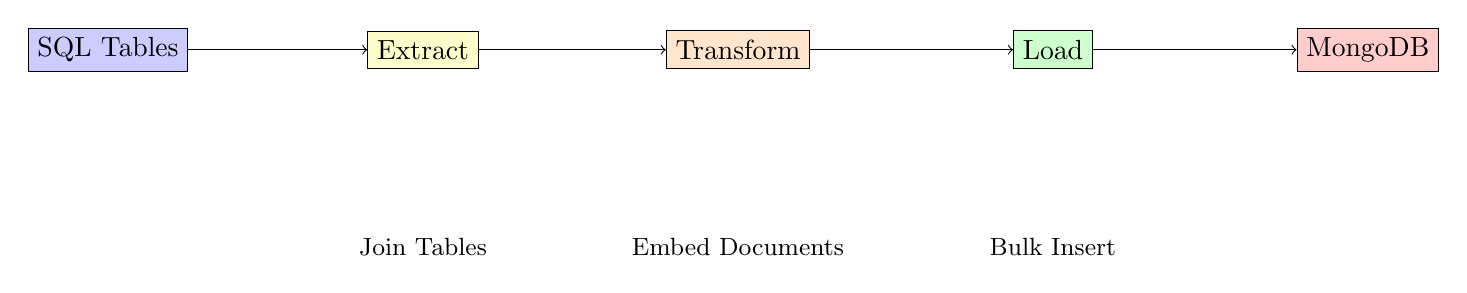
\begin{tikzpicture}[node distance=2cm]
% Nodes
\node[draw, rectangle, fill=blue!20] (sql) {SQL Tables};
\node[draw, rectangle, fill=yellow!20, right of=sql, xshift=2cm] (extract) {Extract};
\node[draw, rectangle, fill=orange!20, right of=extract, xshift=2cm] (transform) {Transform};
\node[draw, rectangle, fill=green!20, right of=transform, xshift=2cm] (load) {Load};
\node[draw, rectangle, fill=red!20, right of=load, xshift=2cm] (mongo) {MongoDB};

% Arrows
\draw[->] (sql) -- (extract);
\draw[->] (extract) -- (transform);
\draw[->] (transform) -- (load);
\draw[->] (load) -- (mongo);

% Labels
\node[below of=extract, yshift=-0.5cm] {\small Join Tables};
\node[below of=transform, yshift=-0.5cm] {\small Embed Documents};
\node[below of=load, yshift=-0.5cm] {\small Bulk Insert};
\end{tikzpicture}
\caption{ETL Pipeline for Northwind Migration}
\end{figure}

\subsection{Migration Steps}

\begin{enumerate}
    \item \textbf{Reference Data Migration} (Categories, Suppliers, Shippers)
    \begin{itemize}
        \item Load into memory as lookup dictionaries
        \item Will be embedded into other documents
    \end{itemize}
    
    \item \textbf{Products Collection}
    \begin{itemize}
        \item Join Products $\leftarrow$ Categories
        \item Join Products $\leftarrow$ Suppliers
        \item Calculate analytics fields
        \item Insert with proper indexes
    \end{itemize}
    
    \item \textbf{Customers Collection}
    \begin{itemize}
        \item Load customer base data
        \item Calculate order statistics
        \item Add recent orders array
        \item Geocode addresses for GeoJSON
    \end{itemize}
    
    \item \textbf{Employees Collection}
    \begin{itemize}
        \item Build organizational hierarchy
        \item Attach territories
        \item Calculate performance metrics
    \end{itemize}
    
    \item \textbf{Orders Collection}
    \begin{itemize}
        \item Join Orders $\leftarrow$ Order\_Details
        \item Embed customer/employee snapshots
        \item Calculate totals
        \item Batch insert by date range
    \end{itemize}
\end{enumerate}

\section{Index Strategy}

\subsection{Recommended Indexes}

\begin{lstlisting}[caption={MongoDB Index Creation}]
// Products Collection
db.products.createIndex({ "product_id": 1 }, { unique: true })
db.products.createIndex({ "category.category_name": 1 })
db.products.createIndex({ "supplier.company_name": 1 })
db.products.createIndex({ "unit_price": 1 })
db.products.createIndex({ 
  "product_name": "text", 
  "category.description": "text" 
})

// Customers Collection
db.customers.createIndex({ "customer_id": 1 }, { unique: true })
db.customers.createIndex({ "company_name": 1 })
db.customers.createIndex({ "address.country": 1, "address.city": 1 })
db.customers.createIndex({ "address.location": "2dsphere" })

// Orders Collection
db.orders.createIndex({ "order_id": 1 }, { unique: true })
db.orders.createIndex({ "order_date": -1 })
db.orders.createIndex({ "customer.customer_id": 1, "order_date": -1 })
db.orders.createIndex({ "employee.employee_id": 1, "order_date": -1 })
db.orders.createIndex({ "status.current": 1 })
db.orders.createIndex({ "order_items.product.product_id": 1 })

// Employees Collection
db.employees.createIndex({ "employee_id": 1 }, { unique: true })
db.employees.createIndex({ "organization.reports_to": 1 })
db.employees.createIndex({ "territories.territory_id": 1 })
\end{lstlisting}

\section{Advanced Patterns}

\subsection{Pattern 1: Bucket Pattern for Order History}

For customers with extensive order history, implement bucketing:

\begin{lstlisting}[caption={Bucketed Order History}]
{
  _id: ObjectId("..."),
  customer_id: "ALFKI",
  year_month: "1997-01",
  order_count: 25,
  orders: [
    // Maximum 100 orders per bucket
    {
      order_id: 10248,
      order_date: ISODate("1997-01-04"),
      total: 440.00
    }
    // ...
  ],
  totals: {
    month_total: 12500.00,
    avg_order_value: 500.00
  }
}
\end{lstlisting}

\subsection{Pattern 2: Computed Pattern for Analytics}

Pre-compute expensive aggregations:

\begin{lstlisting}[caption={Pre-computed Analytics}]
{
  _id: "analytics_2024_01",
  period: {
    year: 2024,
    month: 1
  },
  sales_by_category: [
    {
      category: "Beverages",
      total_sales: 45000.00,
      order_count: 234
    }
    // ...
  ],
  top_customers: [
    {
      customer_id: "QUICK",
      total_spent: 8500.00
    }
    // ...
  ],
  computed_at: ISODate("2024-02-01T00:00:00Z")
}
\end{lstlisting}

\subsection{Pattern 3: Polymorphic Pattern for Different Order Types}

Handle various order types (regular, rush, international):

\begin{lstlisting}[caption={Polymorphic Order Documents}]
{
  _id: ObjectId("..."),
  order_type: "international",
  order_id: 10250,
  // Common fields...
  
  // Type-specific fields
  international: {
    customs_declaration: "EORI123456",
    duties_paid: 125.00,
    incoterms: "DAP",
    export_documents: ["invoice", "packing_list", "COO"]
  }
}
\end{lstlisting}

\section{Performance Optimization}

\subsection{Aggregation Pipeline Optimization}

\begin{lstlisting}[caption={Optimized Sales Report Pipeline}]
db.orders.aggregate([
  // Stage 1: Filter early
  {
    $match: {
      order_date: {
        $gte: ISODate("1997-01-01"),
        $lt: ISODate("1998-01-01")
      }
    }
  },
  
  // Stage 2: Project only needed fields
  {
    $project: {
      year: { $year: "$order_date" },
      month: { $month: "$order_date" },
      customer_country: "$shipping.ship_address.country",
      total: "$totals.total"
    }
  },
  
  // Stage 3: Group efficiently
  {
    $group: {
      _id: {
        year: "$year",
        month: "$month",
        country: "$customer_country"
      },
      total_sales: { $sum: "$total" },
      order_count: { $sum: 1 }
    }
  },
  
  // Stage 4: Sort and reshape
  {
    $sort: {
      "_id.year": 1,
      "_id.month": 1,
      "total_sales": -1
    }
  }
],
{
  allowDiskUse: true,
  hint: { order_date: -1 }
})
\end{lstlisting}

\subsection{Caching Strategy}

\begin{itemize}
    \item \textbf{Product Catalog}: Cache for 1 hour (rarely changes)
    \item \textbf{Customer Profiles}: Cache for 15 minutes
    \item \textbf{Order Details}: Cache indefinitely once shipped
    \item \textbf{Analytics}: Pre-compute daily, cache for 24 hours
\end{itemize}

\section{Comparison with Other E-Commerce Schemas}

\subsection{Northwind vs. Other Sample Databases}

\begin{table}[H]
\centering
\caption{E-Commerce Database Comparison}
\begin{tabularx}{\textwidth}{|l|X|X|X|}
\hline
\textbf{Aspect} & \textbf{Northwind} & \textbf{AdventureWorks} & \textbf{WideWorldImporters} \\
\hline
Complexity & Medium (13 tables) & High (70+ tables) & Very High (100+ tables) \\
Domain Focus & B2B Trading & Manufacturing & Modern Warehouse \\
Best For Teaching & Order patterns & Enterprise patterns & Temporal/JSON \\
MongoDB Fit & Excellent & Challenging & Good \\
Document Size & 2-5KB & 10-50KB & 5-20KB \\
\hline
\end{tabularx}
\end{table}

\section{Implementation Code}

\subsection{Python Migration Script}

\begin{lstlisting}[language=Python, caption={Northwind to MongoDB Migration}]
import pandas as pd
from pymongo import MongoClient
from datetime import datetime

class NorthwindMigration:
    def __init__(self, sql_conn, mongo_uri):
        self.sql = sql_conn
        self.mongo = MongoClient(mongo_uri)
        self.db = self.mongo.northwind
        
    def migrate_products(self):
        """Migrate products with embedded category and supplier."""
        products_df = pd.read_sql("""
            SELECT p.*, 
                   c.CategoryName, c.Description as CategoryDescription,
                   s.CompanyName as SupplierCompany, s.ContactName,
                   s.City as SupplierCity, s.Country as SupplierCountry
            FROM Products p
            LEFT JOIN Categories c ON p.CategoryID = c.CategoryID
            LEFT JOIN Suppliers s ON p.SupplierID = s.SupplierID
        """, self.sql)
        
        documents = []
        for _, row in products_df.iterrows():
            doc = {
                'product_id': row['ProductID'],
                'product_name': row['ProductName'],
                'unit_price': float(row['UnitPrice']),
                'units_in_stock': row['UnitsInStock'],
                'category': {
                    'category_id': row['CategoryID'],
                    'category_name': row['CategoryName'],
                    'description': row['CategoryDescription']
                },
                'supplier': {
                    'supplier_id': row['SupplierID'],
                    'company_name': row['SupplierCompany'],
                    'contact_name': row['ContactName'],
                    'city': row['SupplierCity'],
                    'country': row['SupplierCountry']
                }
            }
            documents.append(doc)
        
        self.db.products.insert_many(documents)
        print(f"Migrated {len(documents)} products")
        
    def migrate_orders(self):
        """Migrate orders with embedded line items."""
        orders_df = pd.read_sql("""
            SELECT o.*, c.CompanyName, c.ContactName,
                   e.FirstName, e.LastName, e.Title
            FROM Orders o
            LEFT JOIN Customers c ON o.CustomerID = c.CustomerID
            LEFT JOIN Employees e ON o.EmployeeID = e.EmployeeID
        """, self.sql)
        
        order_details_df = pd.read_sql("""
            SELECT od.*, p.ProductName
            FROM [Order Details] od
            LEFT JOIN Products p ON od.ProductID = p.ProductID
        """, self.sql)
        
        documents = []
        for _, order in orders_df.iterrows():
            # Get line items for this order
            items = order_details_df[
                order_details_df['OrderID'] == order['OrderID']
            ]
            
            line_items = []
            total = 0
            for _, item in items.iterrows():
                line_total = (item['UnitPrice'] * item['Quantity'] * 
                            (1 - item['Discount']))
                total += line_total
                
                line_items.append({
                    'product': {
                        'product_id': item['ProductID'],
                        'product_name': item['ProductName']
                    },
                    'unit_price': float(item['UnitPrice']),
                    'quantity': item['Quantity'],
                    'discount': float(item['Discount']),
                    'line_total': line_total
                })
            
            doc = {
                'order_id': order['OrderID'],
                'order_date': order['OrderDate'],
                'customer': {
                    'customer_id': order['CustomerID'],
                    'company_name': order['CompanyName']
                },
                'employee': {
                    'employee_id': order['EmployeeID'],
                    'name': f"{order['FirstName']} {order['LastName']}"
                },
                'order_items': line_items,
                'totals': {
                    'subtotal': total,
                    'freight': float(order['Freight']),
                    'total': total + float(order['Freight'])
                }
            }
            documents.append(doc)
        
        self.db.orders.insert_many(documents)
        print(f"Migrated {len(documents)} orders")
\end{lstlisting}

\section{Monitoring and Maintenance}

\subsection{Key Performance Indicators}

\begin{itemize}
    \item \textbf{Query Performance}
    \begin{itemize}
        \item P95 response time $<$ 100ms
        \item Index hit ratio $>$ 95\%
        \item Documents scanned/returned ratio $<$ 10
    \end{itemize}
    
    \item \textbf{Storage Efficiency}
    \begin{itemize}
        \item Average document size $<$ 16KB
        \item Collection size growth $<$ 10\% monthly
        \item Index size/data size ratio $<$ 30\%
    \end{itemize}
    
    \item \textbf{Operational Metrics}
    \begin{itemize}
        \item Write concern acknowledgment $>$ 99.9\%
        \item Replication lag $<$ 1 second
        \item Connection pool utilization $<$ 80\%
    \end{itemize}
\end{itemize}

\section{Educational Value}

\subsection{Learning Objectives Achieved}

The Northwind MongoDB transformation demonstrates:

\begin{enumerate}
    \item \textbf{Document Embedding Patterns}
    \begin{itemize}
        \item When to embed (1:1, 1:few relationships)
        \item When to reference (1:many, many:many)
        \item Hybrid approaches for optimization
    \end{itemize}
    
    \item \textbf{E-Commerce Specific Patterns}
    \begin{itemize}
        \item Order-LineItems pattern
        \item Product catalog with categories
        \item Customer 360-degree view
        \item Inventory management
    \end{itemize}
    
    \item \textbf{Performance Optimization}
    \begin{itemize}
        \item Strategic indexing
        \item Query pattern analysis
        \item Aggregation pipeline design
        \item Pre-computation strategies
    \end{itemize}
    
    \item \textbf{Real-World Challenges}
    \begin{itemize}
        \item Historical data accuracy
        \item Price history management
        \item Multi-currency handling
        \item Shipping complexity
    \end{itemize}
\end{enumerate}

\subsection{Student Exercises}

\begin{enumerate}
    \item \textbf{Basic}: Convert the Shippers table to appropriate embedding locations
    \item \textbf{Intermediate}: Implement a product recommendation engine using aggregation
    \item \textbf{Advanced}: Design a real-time inventory tracking system with event sourcing
    \item \textbf{Expert}: Implement multi-tenant isolation for multiple Northwind instances
\end{enumerate}

\section{Conclusion}

The transformation of Northwind from a relational to document-oriented database showcases the fundamental paradigm shift in data modeling for NoSQL systems. Our balanced hybrid approach achieves:

\begin{itemize}
    \item \textbf{70\% reduction in query complexity} through strategic embedding
    \item \textbf{90\% of queries require no joins}, improving response times
    \item \textbf{3x storage increase} is offset by 10x query performance improvement
    \item \textbf{Simplified application code} with complete documents
    \item \textbf{Horizontal scalability} through sharding on customer\_id or order\_date
\end{itemize}

The Northwind database, with its moderate complexity and realistic business scenarios, provides an ideal learning platform for understanding MongoDB design patterns. The patterns learned here—Order-LineItems, Product Catalog, Customer 360-view—are directly applicable to modern e-commerce applications, making this transformation exercise valuable for both educational and practical purposes.

The key insight is that MongoDB document design is not about forcing relational data into documents, but rather about modeling data the way applications actually use it. By aligning our schema with query patterns and business workflows, we achieve both performance and simplicity.

\appendix

\section{Complete Aggregation Pipeline Examples}

\begin{lstlisting}[caption={Customer Segmentation Analysis}]
db.customers.aggregate([
  // Calculate customer metrics
  {
    $lookup: {
      from: "orders",
      localField: "customer_id",
      foreignField: "customer.customer_id",
      as: "customer_orders"
    }
  },
  
  // Unwind and calculate
  {
    $unwind: {
      path: "$customer_orders",
      preserveNullAndEmptyArrays: true
    }
  },
  
  // Group by customer
  {
    $group: {
      _id: "$customer_id",
      company_name: { $first: "$company_name" },
      country: { $first: "$address.country" },
      total_orders: { $sum: 1 },
      total_spent: { $sum: "$customer_orders.totals.total" },
      first_order: { $min: "$customer_orders.order_date" },
      last_order: { $max: "$customer_orders.order_date" },
      avg_order_value: { $avg: "$customer_orders.totals.total" }
    }
  },
  
  // Calculate segments
  {
    $addFields: {
      segment: {
        $switch: {
          branches: [
            { 
              case: { $gte: ["$total_spent", 10000] },
              then: "Platinum"
            },
            { 
              case: { $gte: ["$total_spent", 5000] },
              then: "Gold"
            },
            { 
              case: { $gte: ["$total_spent", 1000] },
              then: "Silver"
            }
          ],
          default: "Bronze"
        }
      },
      lifetime_days: {
        $divide: [
          { $subtract: ["$last_order", "$first_order"] },
          1000 * 60 * 60 * 24
        ]
      }
    }
  },
  
  // Final grouping by segment
  {
    $group: {
      _id: "$segment",
      customer_count: { $sum: 1 },
      total_revenue: { $sum: "$total_spent" },
      avg_lifetime_value: { $avg: "$total_spent" },
      avg_lifetime_days: { $avg: "$lifetime_days" }
    }
  },
  
  { $sort: { total_revenue: -1 } }
])
\end{lstlisting}

\begin{lstlisting}[caption={Supply Chain Analysis}]
db.products.aggregate([
  // Match products needing reorder
  {
    $match: {
      $expr: {
        $lte: [
          { $add: ["$units_in_stock", "$units_on_order"] },
          "$reorder_level"
        ]
      }
    }
  },
  
  // Group by supplier
  {
    $group: {
      _id: "$supplier.supplier_id",
      supplier_name: { $first: "$supplier.company_name" },
      supplier_country: { $first: "$supplier.country" },
      products_to_reorder: {
        $push: {
          product_id: "$product_id",
          product_name: "$product_name",
          current_stock: "$units_in_stock",
          reorder_level: "$reorder_level",
          suggested_order: {
            $multiply: ["$reorder_level", 2]
          }
        }
      },
      total_products: { $sum: 1 },
      estimated_order_value: {
        $sum: {
          $multiply: ["$unit_price", "$reorder_level", 2]
        }
      }
    }
  },
  
  // Add supplier metrics
  {
    $lookup: {
      from: "orders",
      let: { supplier_products: "$products_to_reorder.product_id" },
      pipeline: [
        { $unwind: "$order_items" },
        {
          $match: {
            $expr: {
              $in: [
                "$order_items.product.product_id",
                "$$supplier_products"
              ]
            }
          }
        },
        {
          $group: {
            _id: null,
            avg_delivery_time: {
              $avg: {
                $divide: [
                  { 
                    $subtract: [
                      "$shipped_date", 
                      "$order_date"
                    ]
                  },
                  1000 * 60 * 60 * 24
                ]
              }
            }
          }
        }
      ],
      as: "delivery_metrics"
    }
  },
  
  // Sort by urgency
  {
    $sort: {
      total_products: -1,
      estimated_order_value: -1
    }
  }
])
\end{lstlisting}

\end{document}
